%!TEX root = _DaBa.tex
\chapter{Prototypes}
\label{cha:Prototypes}
This chapter will describe the implementation of a C2C application on three different devices. These devices are an Android Device, a Windows Phone and a rasberry pi.

\section{Android}
Since Android 4.0, devices with appropriate hardware are allowed to connect directly to each other over WI-FI P2P without an access point between them. According to the official Android Wi-Fi Peer-to-Peer documentation, Android's P2P framework complies with the WI-FI Alliances' WI-FI Direct certification program. With the usage of this API you are able to discover and connect to other devices when they support WI-FI P2P.  According to documentations the advantage of WI-FI P2P besides Bluetooth or similar connection types is a fast connection across distances much longer than others, see table \ref{table:Wi-Fi Direct}. This allows applications a fast exchange of data between multiple users, which could be useful for applications such as multiplayer games, photosharing applications and in general, all applications which are relying on a fast connection between a long distance.\footnote{\label{foot:1}http://developer.android.com/guide/topics/connectivity/wifip2p.html}

\subsection*{Prototype Implementation}
\label{subsec:AndroidPrototype}
In regard to the Car2Car project an Android application which tests the reliability and the functions of the WI-FI P2P APIs was developed. In light of the idea behind the Car2Car project and the ability of modern Android phones, to track the location of a user, this subchapter will show the results of the simple WI-FI P2P and GPS prototype.
The simple prototype discover available peers, after a successful connection it  sends the GPS location of the user to all connected peers. All peers mark the position of the other devices on the included google maps map with a marker. The picture below shows the design of the prototype application and describes the different sections.

\begin{figure}[ht]
	\centering
  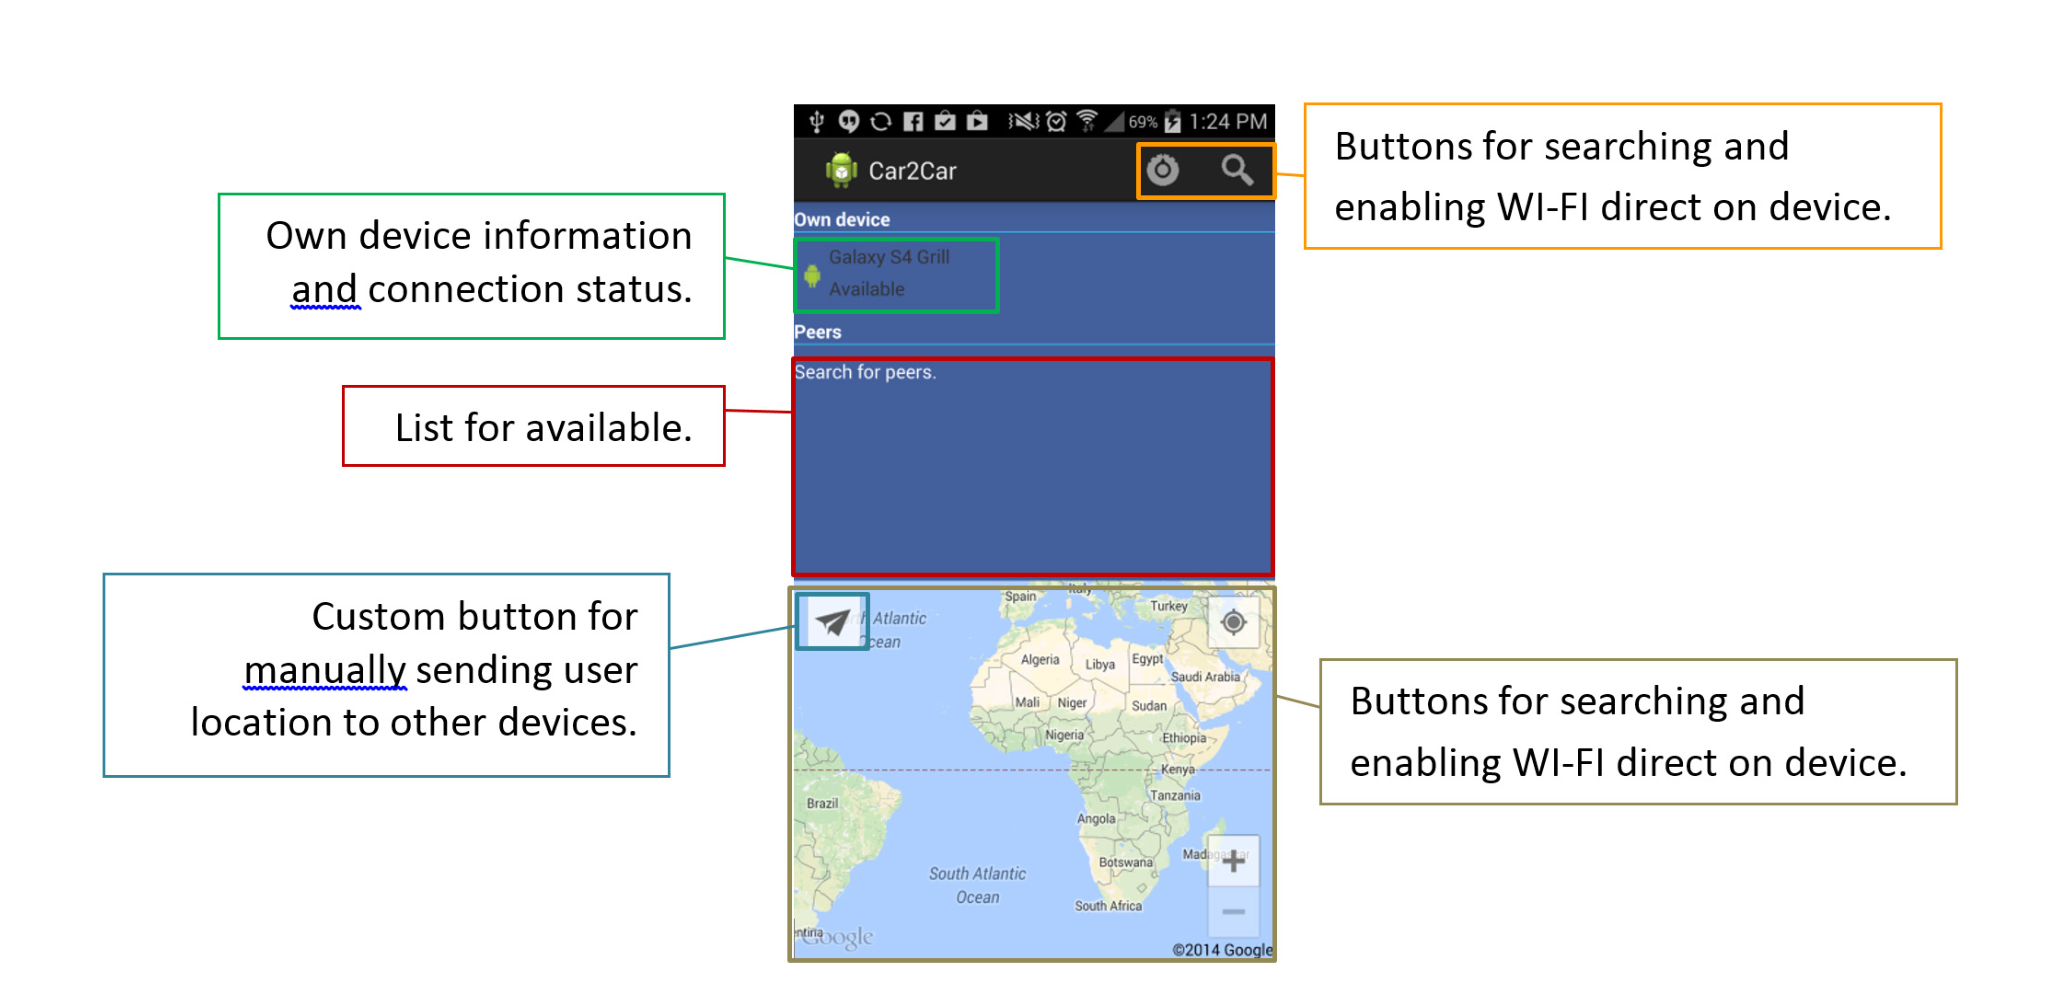
\includegraphics[width=\linewidth]{images/androidScreen1.eps}
	\caption{The figure shows the Android prototype application}
	\label{fig1}
\end{figure}

\noindent When the application is started it automatically begins to search for available peers. Additionally, the user can search manually by pressing the search button in top of the application. The application filters available peers per instance name, which means only other C2C peers are shown. If peers are available they appear immediately in the list view. A user can connect to other devices by clicking on the specific item in the list view. If the connection attempt was successful the invited device will get connection invitation which the user has to accept.  If the other user has accepted the invitation the two application shares their GPS location information. This means, every time the location of the device will change the current GPS information (Longitude and Latitude) will send to all connected peers. In some regions with weak GPS signals it could take several minutes until the application shares their GPS information with the other connected peers. The result of a successful connection is shown in the image below. The position of the other device is marked with a red google marker icon.


\begin{figure}[H]
	\centering
  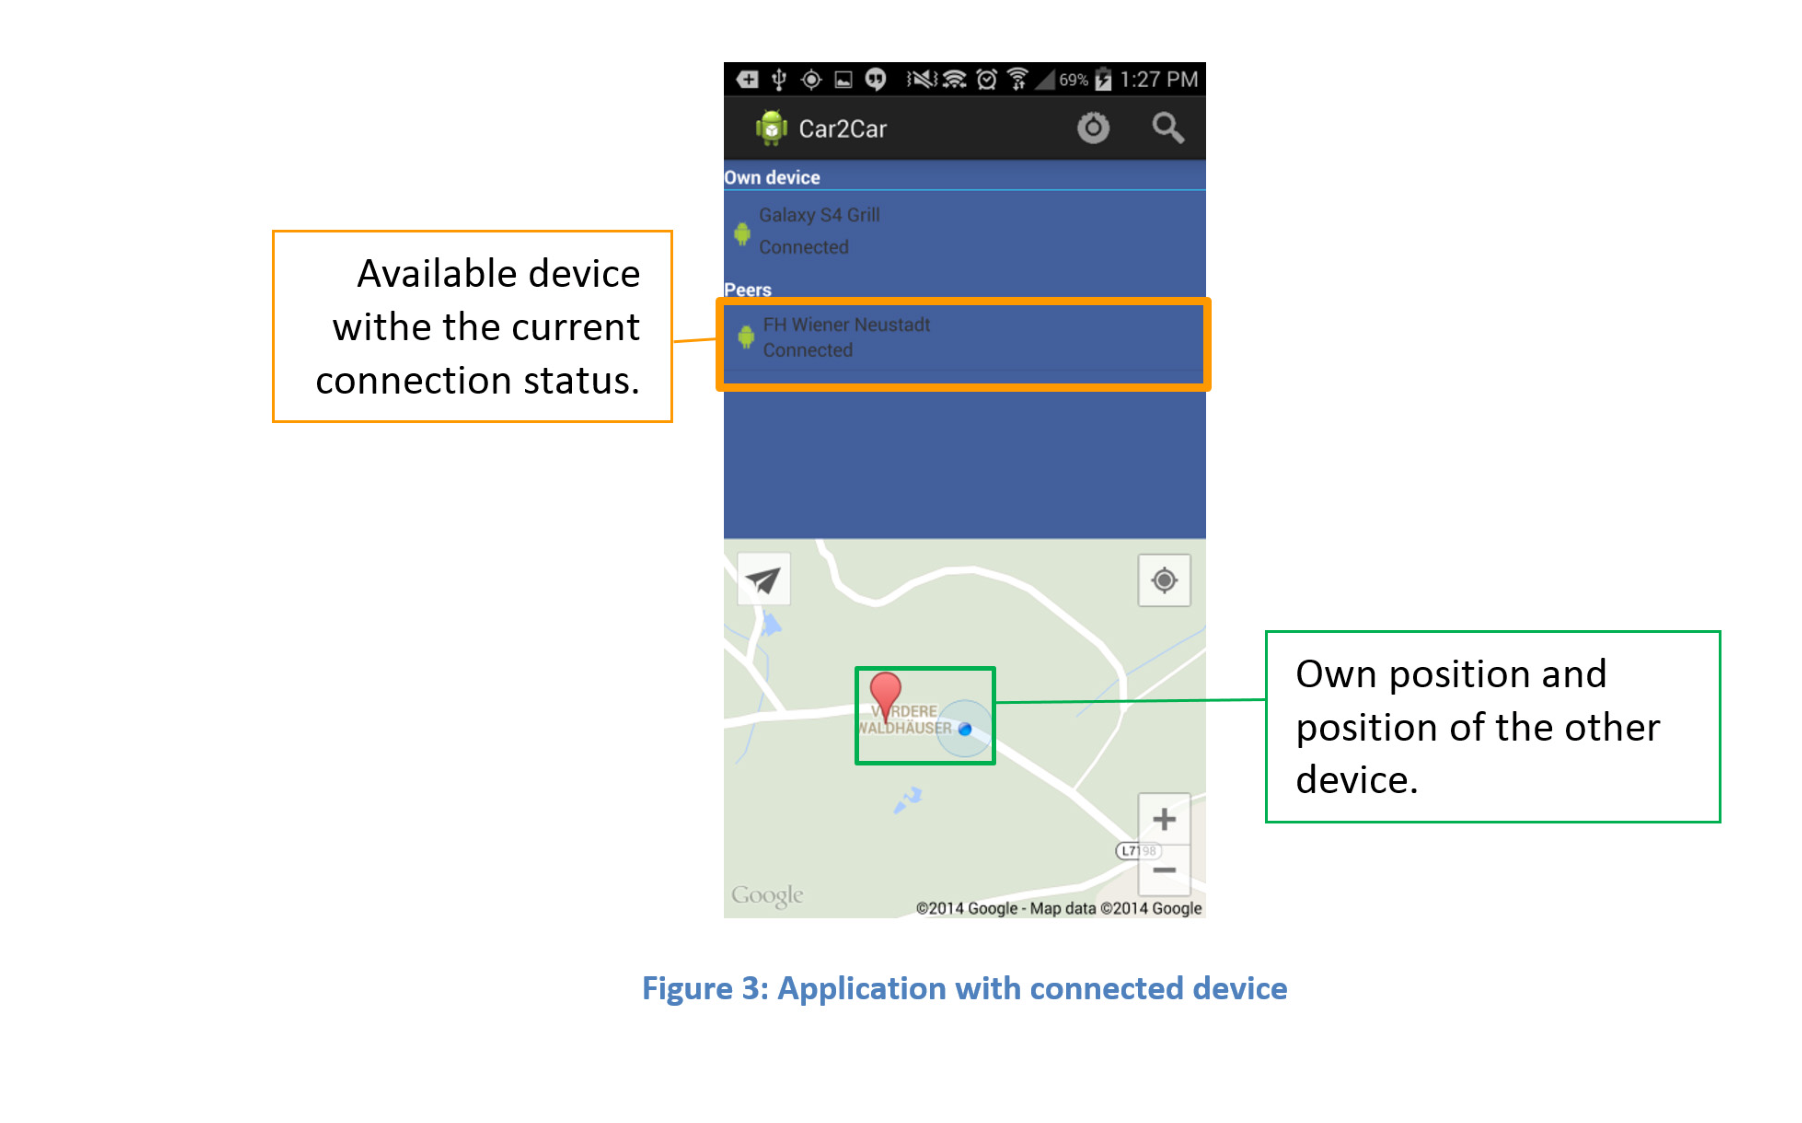
\includegraphics[width=\linewidth]{images/androidScreen2.eps}
	\caption{The figure shows the Android prototype application with a connected device}
	\label{fig1}
\end{figure}

\subsection*{Limitations and Problems}
\label{subsec:AndroidLimitationsProblems}
One of the biggest problems with Androids WI-FI P2P APIs, from the perspective of the C2C project, is the fact that every time a device wants to connect to your smartphone, it requires a confirmation from the user. Of course this had some security backgrounds and it make sense in other scenarios, but it is a major problem for using Android devices and this type of communication in the C2C project.  For obtaining detail information, like the current location or other important details, it is necessary that all devices are connected automatically to each other when they are in the same area. The image below shows an invitation message which shows up on every device which receives a connection request\footnote{\label{foot:2}http://developer.android.com/training/connect-devices-wirelessly/wifi-direct.html}.\newline
 
\begin{figure}[H]
	\centering
  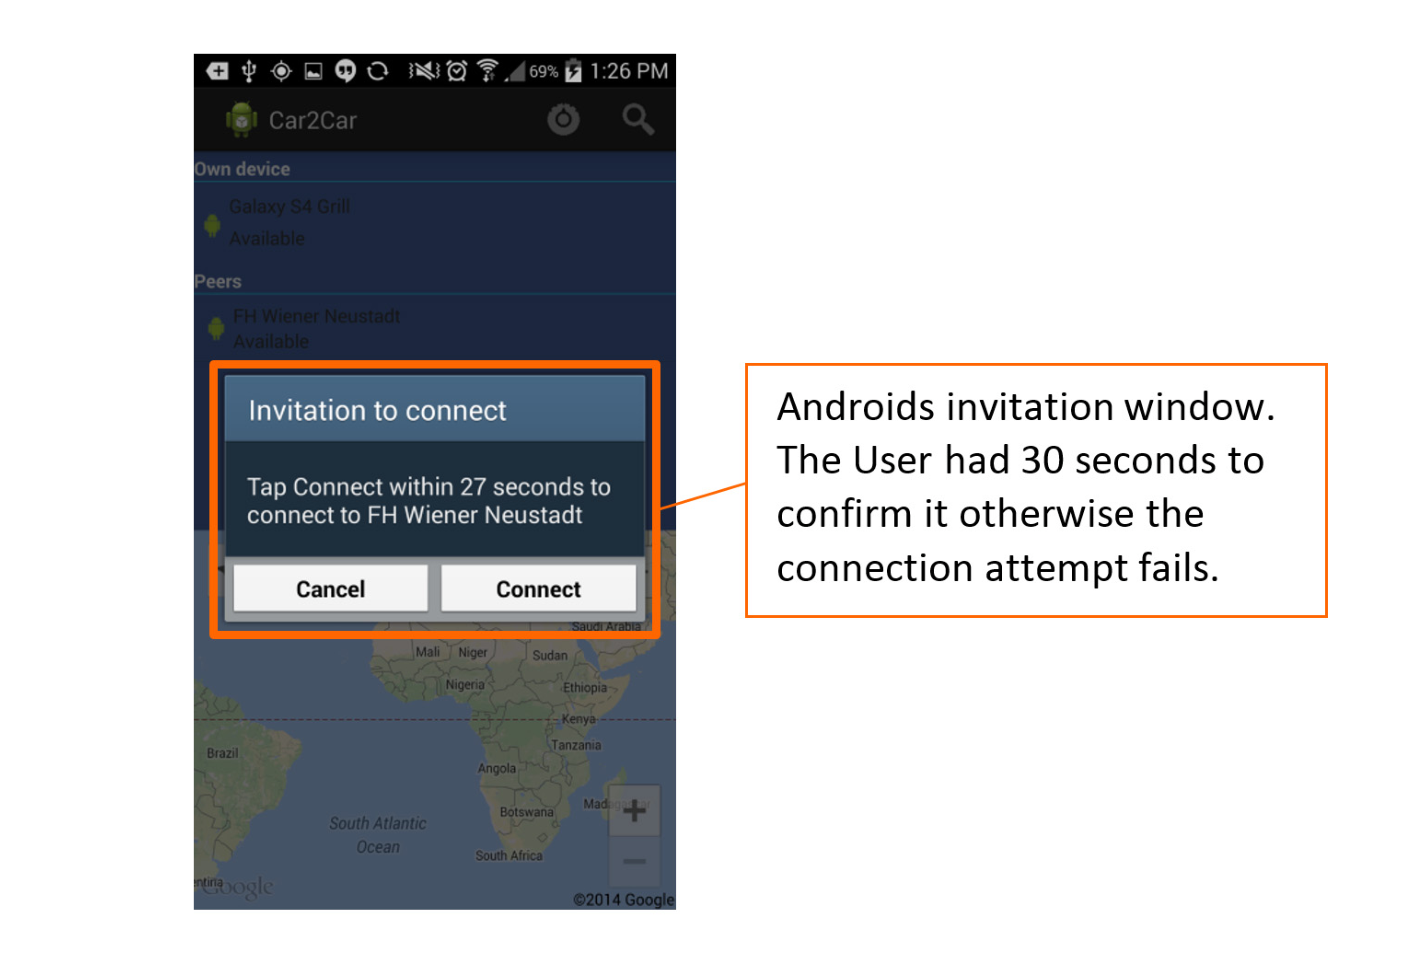
\includegraphics[width=\linewidth,]{images/androidScreen3.eps}
	\caption{The figure shows the Android prototype application with a Wifi P2P connection request}
	\label{fig1}
\end{figure}

\noindent According to the official WI-FI P2P documentation the range of the WI-FI P2P signal could be up to 500 meters. For the Android Car2Car prototype the test devices Samsung Galaxy S4 and Samsung Galaxy S2 Plus was used. It was not possible to confirm the range of 500 meters with the two devices. To test the maximal range of the signal, a few tests on a straight level road were carried out. It was determined that the signal at about 100-120 meters is lost. The tests were performed on foot and by car without any major differences. For a successful reconnect the distance between the devices was about 50-70 meters. The pictures below show the performed tests and describe their results.

\begin{figure}[hb]
	\centering
  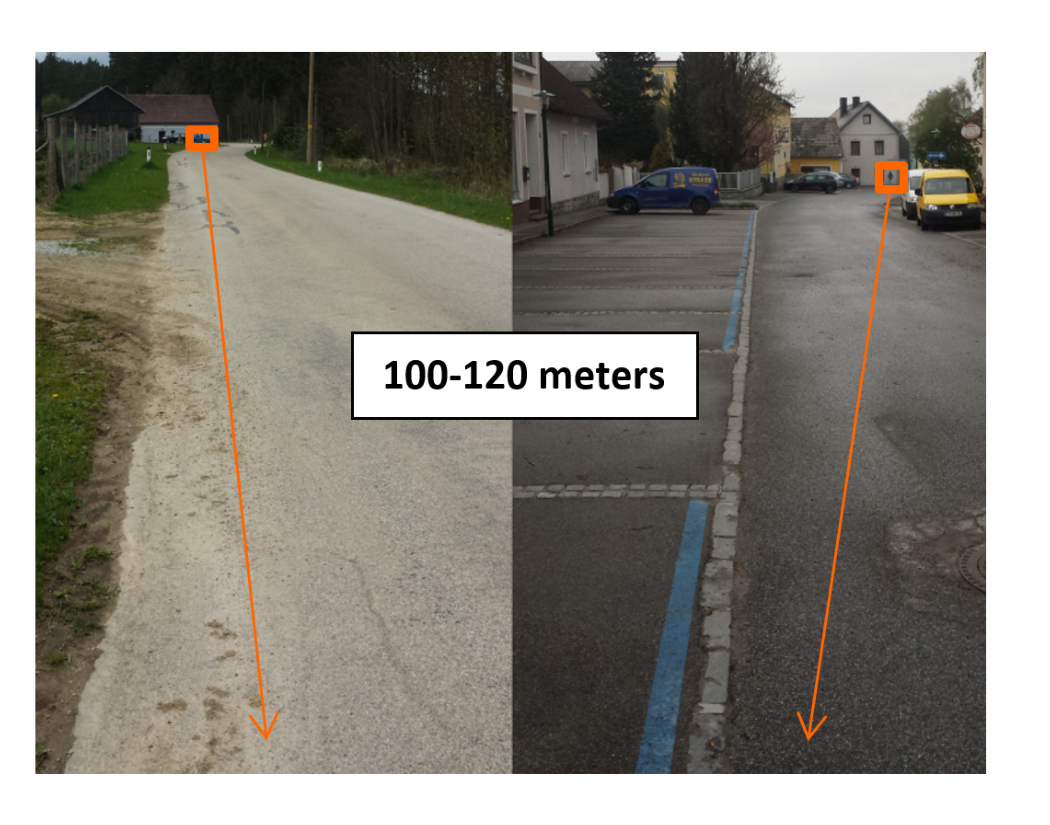
\includegraphics[width=\linewidth]{images/androidScreen4.eps}
	\caption{The figure shows the maximum range of the Wifi P2P signal}
	\label{fig1}
\end{figure}

\begin{figure}[H]
	\centering
  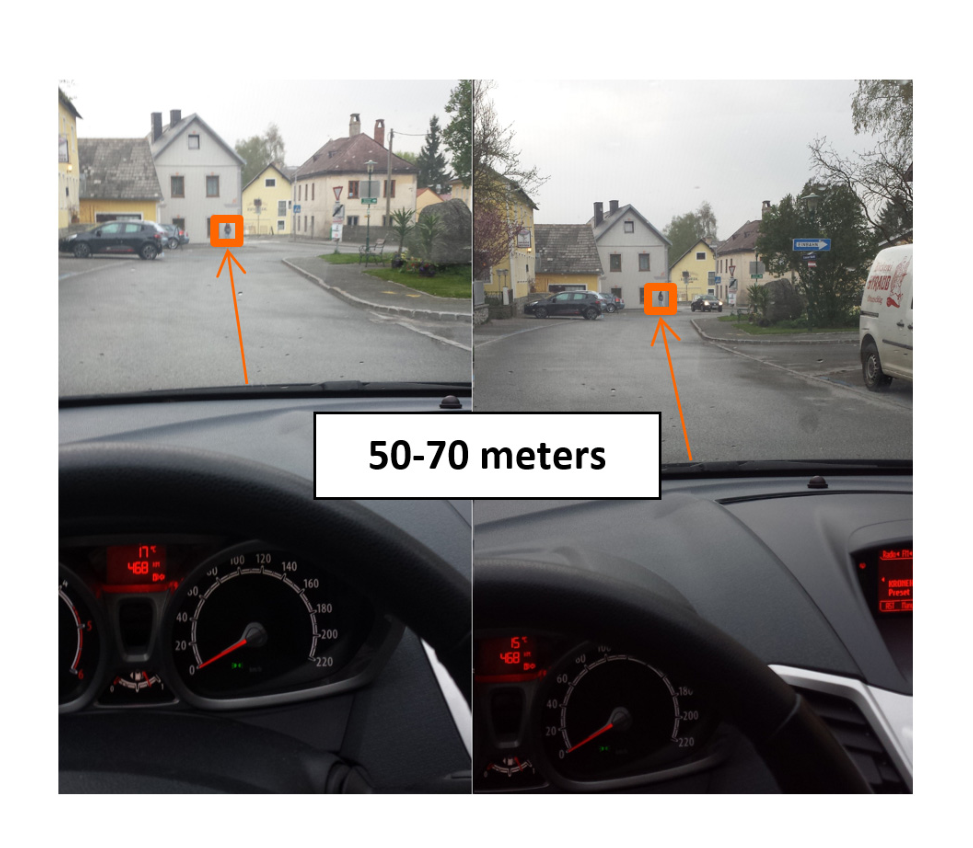
\includegraphics[width=\linewidth]{images/androidScreen5.eps}
	\caption{The figure shows the maximum distance for a successful reconnect}
	\label{fig1}
\end{figure}

\section{Raspberry Pi}
\label{sec:RaspberryPi}
With the right wifi dongle and driver, it is possible to use wifi direct on the Raspberry Pi too. After doing some research on the topic wifi direct on the big mobile plattforms the outcome was not satisfying. The problem was, that espacially iOS and Windows Phone had own proprietary implementations for wifi direct. Therefore the platforms weren't compatible with each other. To guarantee compatibility we had to find an alternative. The Raspberry Pi fits exactly our needs. It would be the wifi direct receiver and sender. Information will be transmitted from the Raspberry Pi to the smartphone, which presents the data to the user. We created a protoype which is able to connect to another wifi direct device. In further implementation it should connect to various devices and broadcast information. Forthermore the problem with accepting wifi direct connections, mentioned in \ref{subsec:AndroidLimitationsProblems}, would be eliminated. In the current prototype it is not implemented, however the automatically connection confirmation could be handled in the connection script.

\subsection*{Prototype Implementation}
\label{subsec:RaspberryPrototype}
A simple prototype was created for the Raspberry Pi, showing the possibility for establishing Wifi direct connections with other Wifi direct enabled devices in case of Car2Car communication. After establishing the connection with the device, a simple UDP-Server is started on the Raspberry Pi and a message will be transmitted over Wifi direct. The Realtek driver includes a console application named P2P UI, which enables Wifi direct and can be used for establishing connections. 

\begin{figure}[!hb]
	\centering
  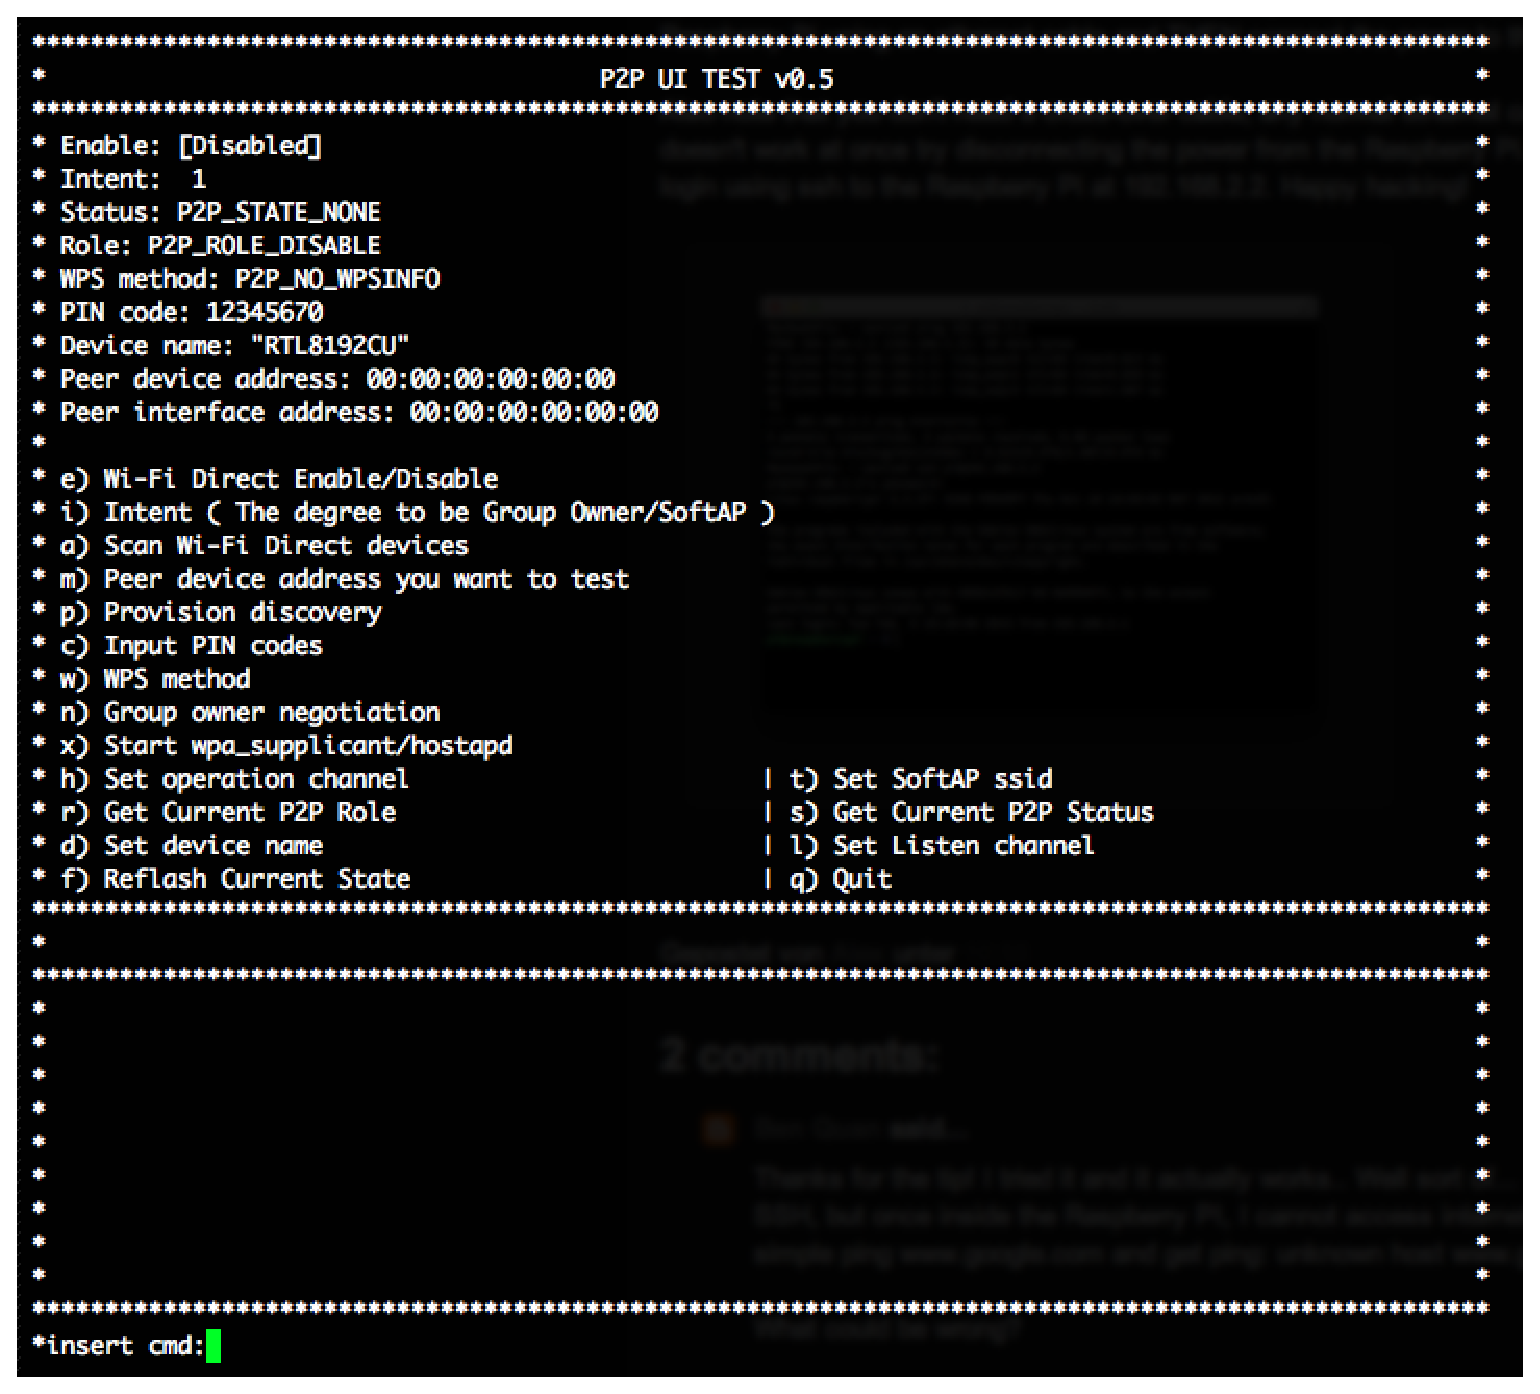
\includegraphics[width=\linewidth]{images/p2p_UI_screenshot.eps}
	\caption{The figure shows the P2P UI application on the Raspberry Pi}
	\label{fig1}
\end{figure}

\noindent After analysing the P2P UI Application, a shell script, which automates the pairing process was created. The user only needs to specify the name of his device and the MAC adress from the device he wants to start the pairing process with. 

\begin{figure}[!hb]
	\centering
  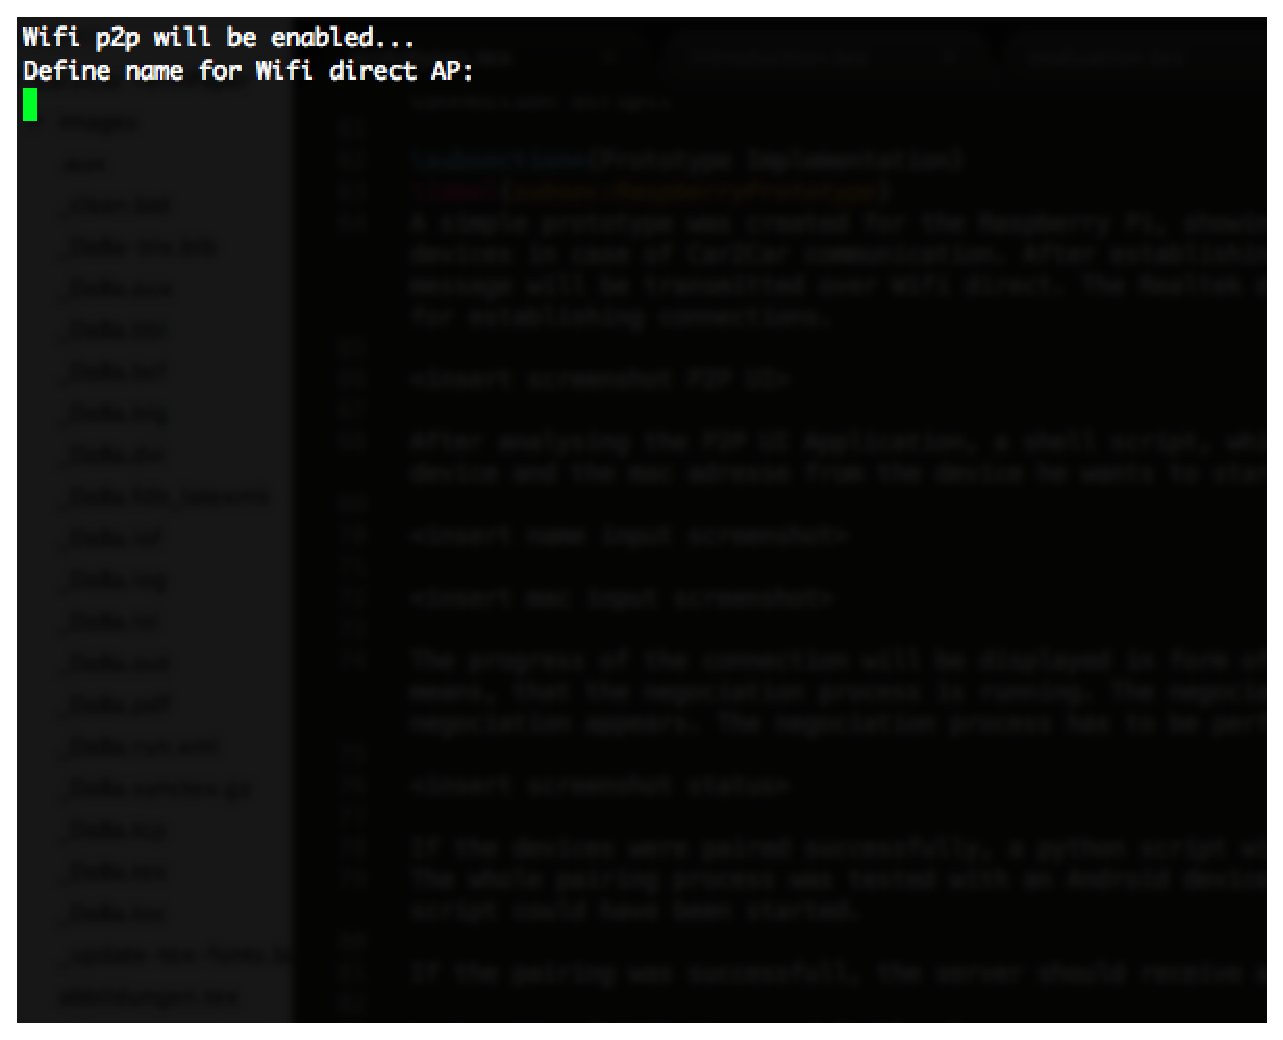
\includegraphics[width=\linewidth]{images/enterName_screenshot.eps}
	\caption{The figure shows the name input in the connect script}
	\label{fig1}
\end{figure}

\begin{figure}[!hb]
	\centering
  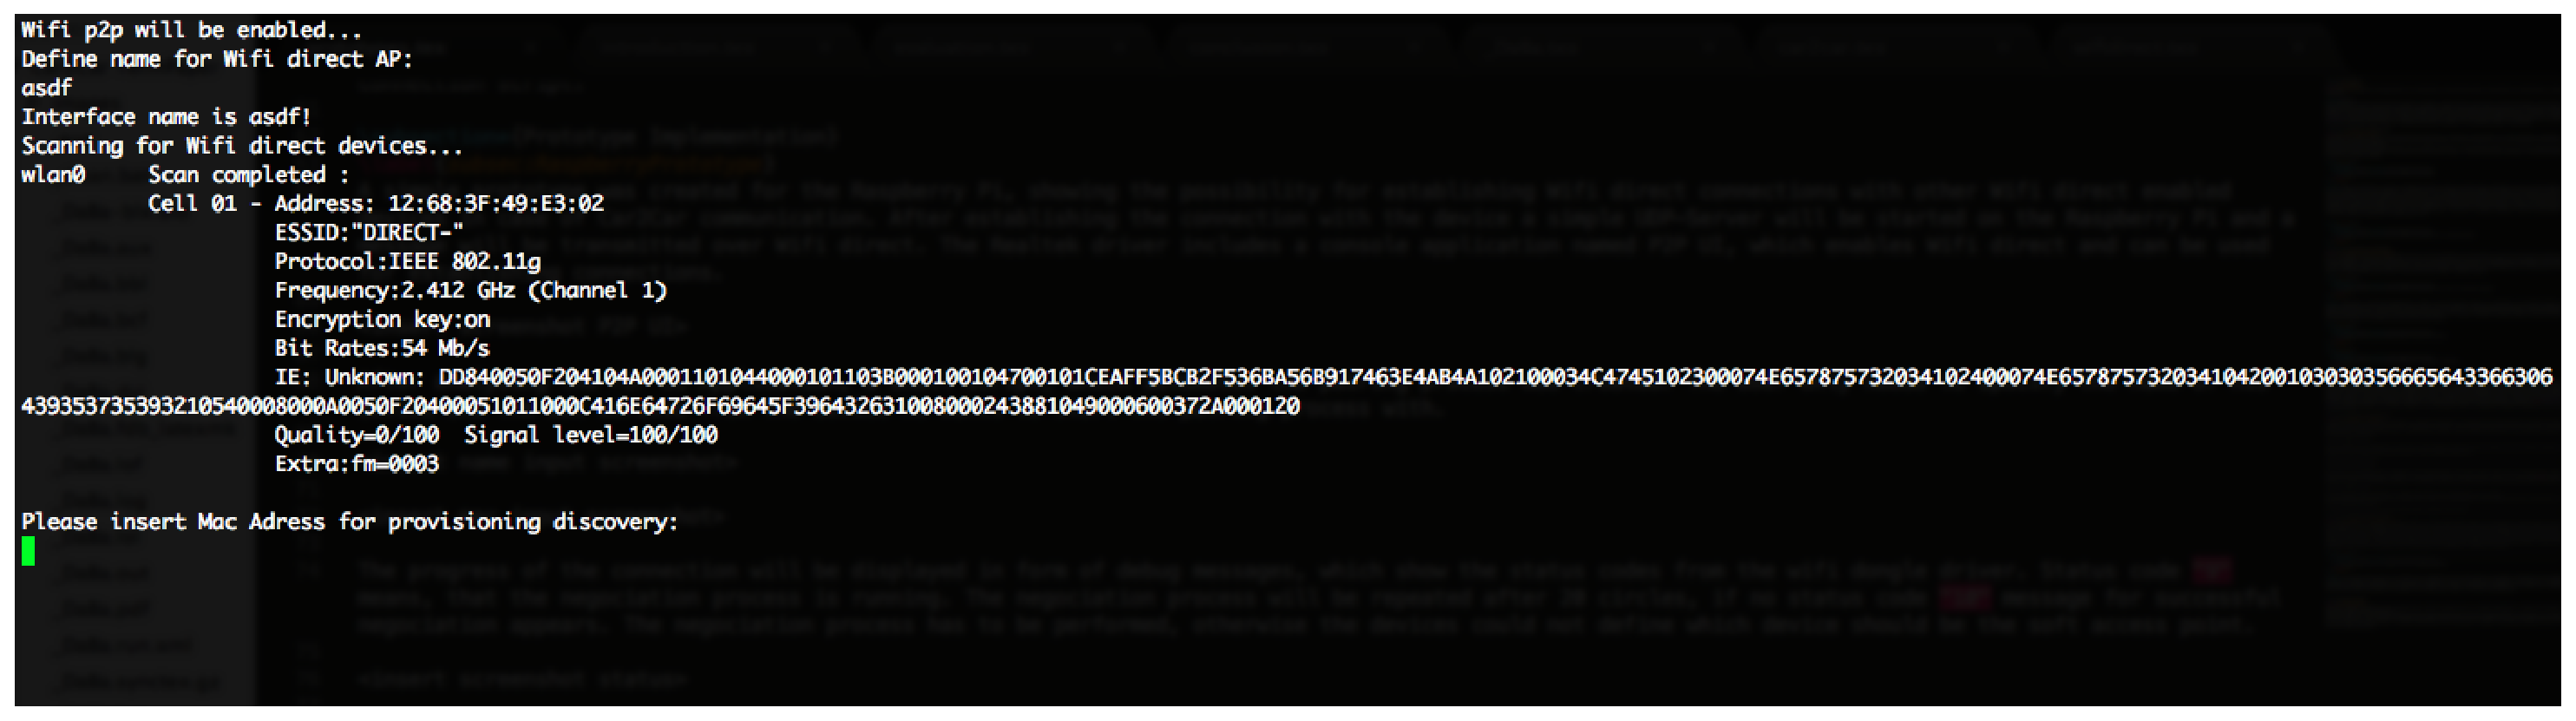
\includegraphics[width=\linewidth]{images/enterMac_screenshot.eps}
	\caption{The figure shows the MAC adress input from the device you wish to connect to}
	\label{fig1}
\end{figure}

\noindent The progress of the connection will be displayed as debug messages, which show the status codes from the wifi dongle driver. Status code "9" means, that the negotiation process is running. The negotiation process will be repeated after 20 circles, if no status code "10" message for successful negotiation appears. The negotiation process has to be performed, otherwise the devices could not define which device should be the soft access point\cite{realtekprogrammingguide}.

\begin{figure}[!hb]
	\centering
  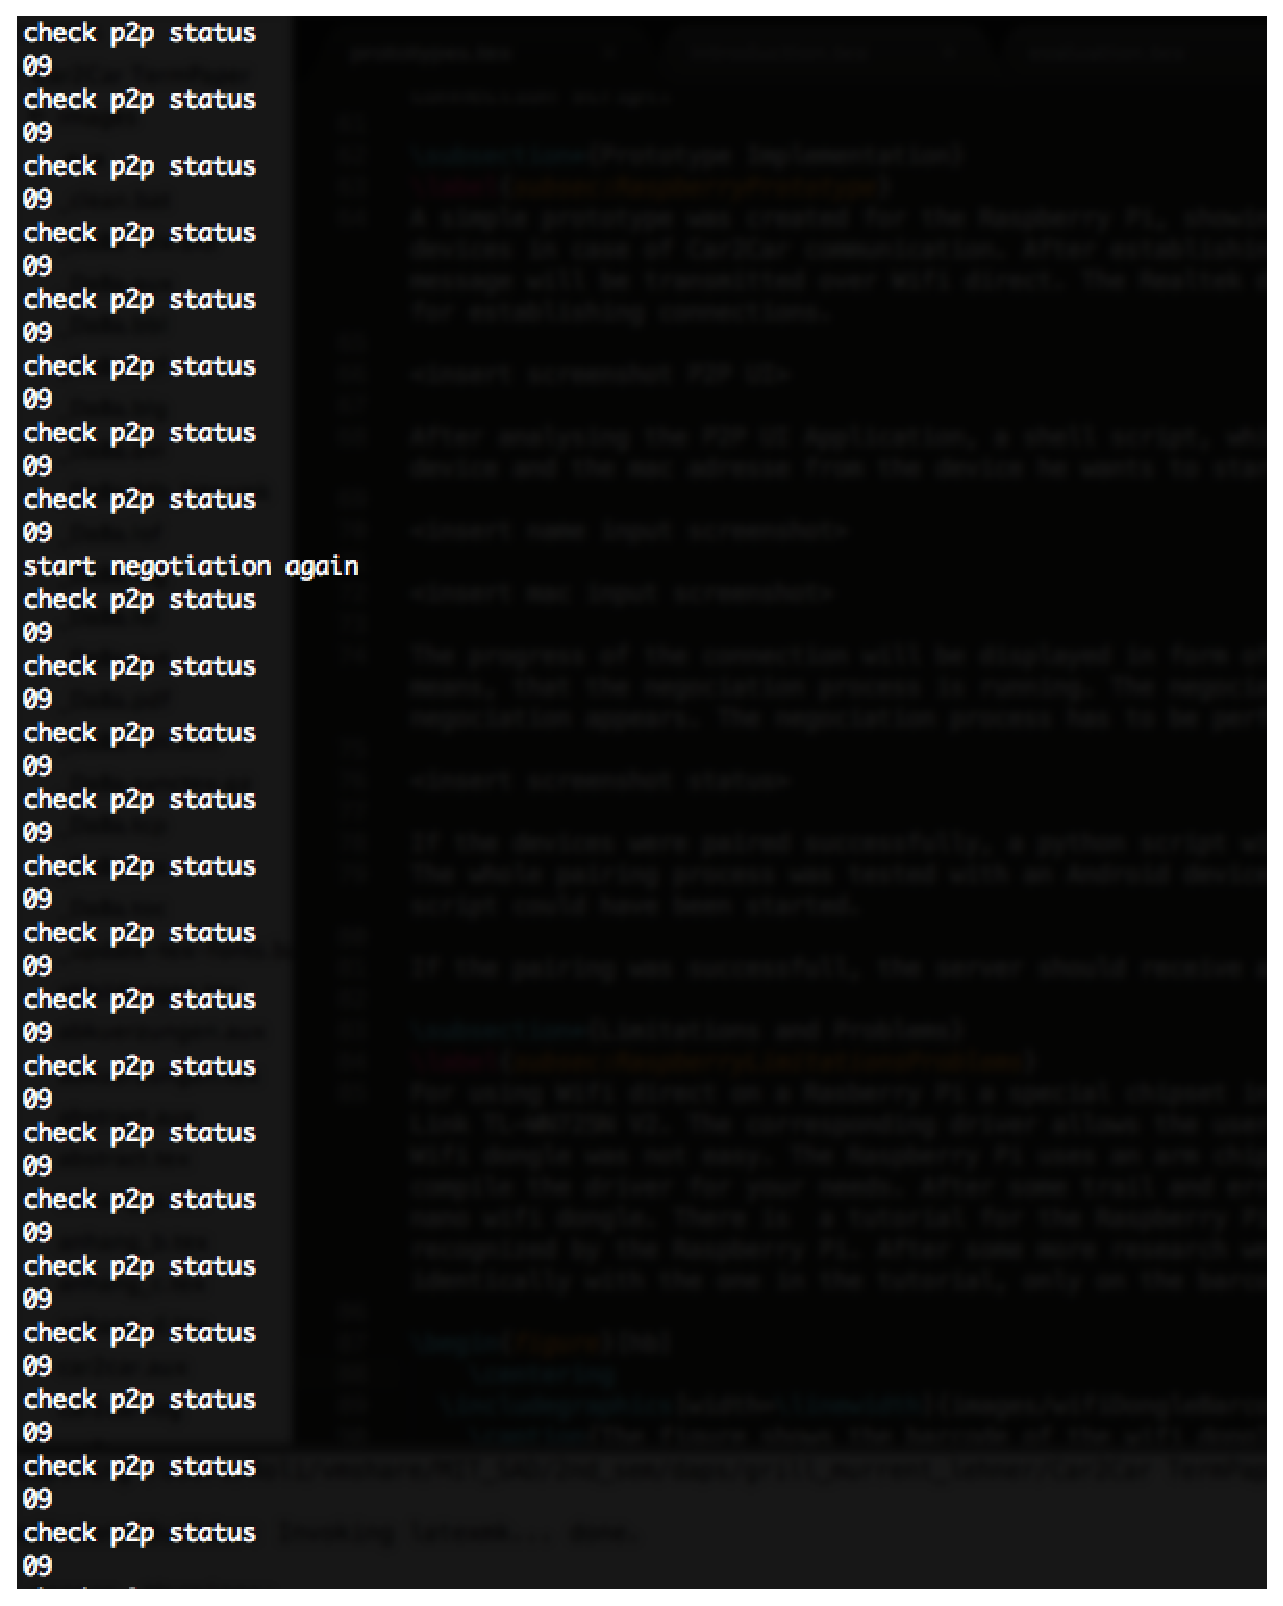
\includegraphics[width=\linewidth]{images/status_screenshot.eps}
	\caption{The figure shows the status output while the negotiation process is in progress}
	\label{fig1}
\end{figure}

\noindent If the devices were paired successfully, a Python script with the server implementation will be started.
The whole pairing process was tested with an Android device (Nexus 4) and the Rapsberry Pi. With an Android application called QPython, the client Python script could have been started.

If the pairing was successfull, the server should receive a message from the client.

\subsection*{Limitations and Problems}
\label{subsec:RaspberryLimitationsProblems}
For using Wifi direct on a Rasberry Pi a special chipset in the Wifi dongle should be used. This prototype uses a Realtek chipset and the Wifi dongle TP-Link TL-WN725N V2. The corresponding driver allows the user to enable Wifi direct compatibility on the chipset. However finding the right driver for the Wifi dongle was not easy. The Raspberry Pi uses an arm chipset, where most of the driver are not precompiled. Either you find a driver or you have to compile the driver for your needs. After some trail and error, the right driver was found to support the Raspberry Pi. Another problem was the TP-Link nano wifi dongle. There is  a tutorial for the Raspberry Pi to enable the wifi direct feature, however it was not possible to use the dongle, it was not recognized by the Raspberry Pi\footnote{http://www.youtube.com/watch?v=6GPv8TfZqe4} \footnote{http://www.youtube.com/watch?v=-HCrfkKeIM0}. After some more research we found out, that the wifi dongle we used was the second version\cite{wifidongleV2}. The name of the dongle was identically with the one in the tutorial, only on the barcode of the packaging was a reference of the model.

\begin{figure}[!hb]
	\centering
  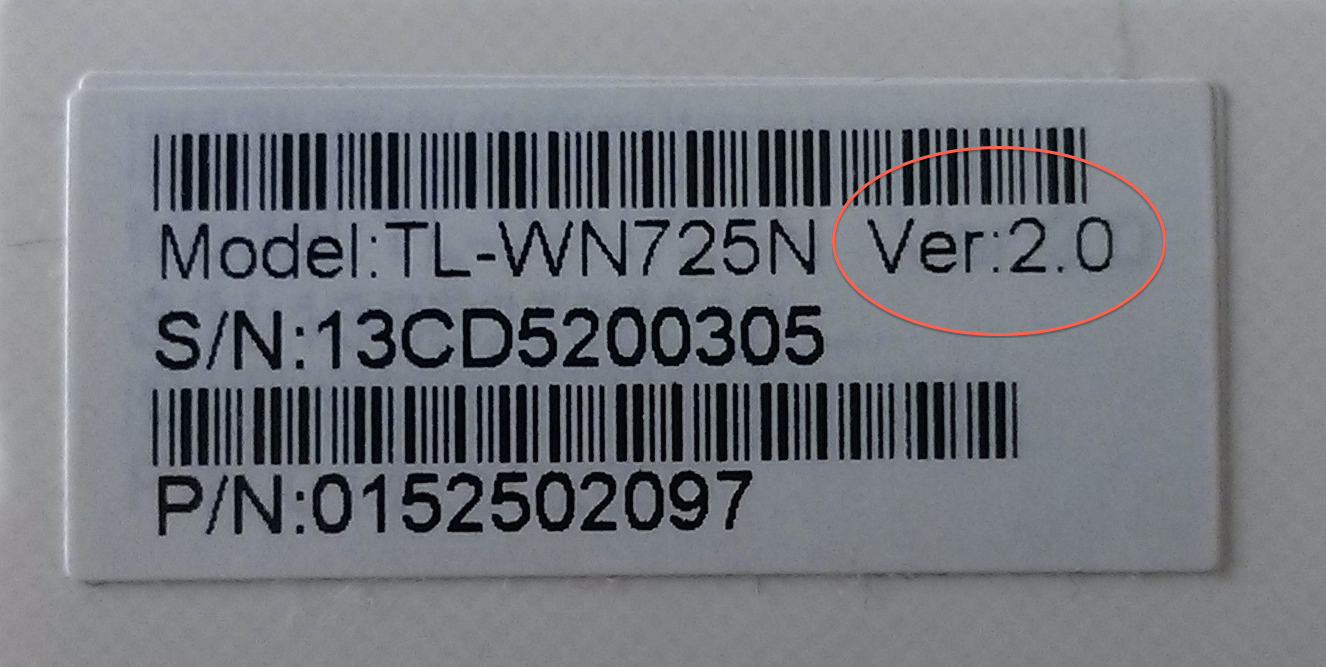
\includegraphics[width=\linewidth]{images/wifiDongleBarcode.eps}
	\caption{The figure shows the barcode of the wifi dongle packaging}
	\label{fig1}
\end{figure}

\noindent The driver which was used in the tutorial was not compatible with the second version of this dongle. Furthermore the whole implementation is not reliable at the moment. Unfortunately it is not possible to garuantee a correct soft access point negotiation on every connect. An investiagtion to fix the problem was initiated, however this goal could not be reached for this paper. Theoratically the Raspberry Pi or Android device, depending which will be the soft access point, should share the IP address from the other device which is in the soft access point mode.


\section{Windows Phone}
\label{sec:WindowsPhone}
Microsoft included Wifi Direct in his new Windows Phone 8.1 SDK, but actually there is no suitable documentation or sample which describes the usage of Wifi Direct within a Windows Phone app.\\
The other option would be to use there Windows.Networking.Proximity namespace which connects two phones directly to each other, but this requires a Bluetooth connection, a WIFI connection and the same app on both devices. Since this is not compatible with any other devices than a Windows Phones, this is, in our case, not the best solution. In the sample app description it is mentioned that an app which communicates via the proximity driver is used if no NFC is supported by the windows phone\footnote{http://code.msdn.microsoft.com/wpapps/Proximity-Sample-88129731}. The biggest disadvantages are that the distance is limited to the Bluetooth distance and that it is not compatible with other phone manufacturer.